\documentclass[12pt, letterpaper, oneside]{article}
\usepackage{amsmath}
\usepackage{amssymb}
\usepackage{csquotes}
\usepackage{float}
\usepackage{hyperref}
\usepackage{tikz}
\usetikzlibrary{arrows, automata, positioning, shapes.geometric}
\usepackage{parskip}
\usepackage{xcolor}

\hypersetup{
  colorlinks=true,
  linkcolor=blue,
  filecolor=magenta,
  urlcolor=blue,
}

\begin{document}

Useful links
\begin{enumerate}
  \item \href{https://latexdraw.com/}{TikZBlog}
        \begin{enumerate}
          \item \href{https://latexdraw.com/tikz-shapes-circle/}{TikZ shapes: Circle}
          \item \href{https://latexdraw.com/how-to-draw-venn-diagrams-in-latex/}{How to draw Venn Diagrams in LaTeX}
          \item \href{https://latexdraw.com/how-to-annotate-an-image-in-latex/}{How to Annotate an Image in LaTeX}
          \item \href{https://latexdraw.com/exploring-tikz-arrows/}{TikZ arrows}
          \item \href{https://hayesall.com/blog/latex-automata/}{LaTeX Finite Automata and State Diagrams with Tikz}
          \item \href{https://tex.stackexchange.com/a/20786/66282}{Which package can be used to draw automata?}
        \end{enumerate}
\end{enumerate}

% =============================================================================
\section{Draw circles}
% =============================================================================

% -----------------------------------------------------------------------------
\subsection{Using ``draw''}
% -----------------------------------------------------------------------------

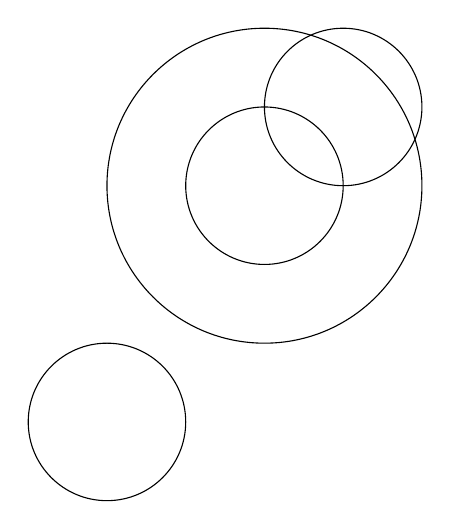
\begin{tikzpicture}
  % "\draw (x, y) circle (r)" draws a circle at the center with coordinates
  % (x,y) and radius r.
  \draw (0, 0) circle (1);
  \draw (0, 0) circle (2);
  \draw (1, 1) circle (1);
  \draw (-2, -3) circle (1);
\end{tikzpicture}

% -----------------------------------------------------------------------------
\subsection{Using ``node''}
% -----------------------------------------------------------------------------

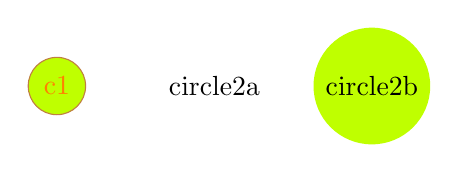
\begin{tikzpicture}
  % This defines a general node.
  \node[
    % Tell tikz to draw the node as a circle.
    circle,
    % Without "draw", the circle is drawn in white so it looks as if the circle
    % is not there, but it is. See "circle2a" ~ "circle2c".
    % The color of "draw" specify the border line color of the circle.
    draw=brown,
    % "text" specifies the text color in the circle.
    text=orange,
    % "fill" specifies the filling color in the circle.
    fill=lime,
  ]
  % The tutorial says this is the node's name. It's not drawn anywhere so I
  % guess it's an internal name to refer to the circle.
  (c1)
  % The center coordinates of the circle.
  at (0, 0)
  % "{}" contains the text to display on the circle.
  % Note that the size of the circle depends on the content in it. For example,
  % "c1" is shorter than "circle2a" and "circle2b" so the circle c1 is smaller
  % than circles c2a and c2b. We can define the minimum size of the circle but
  % TikZ figures out the actual size.
  {c1};
  \node[circle] (c2a) at (2, 0) {circle2a};
  \node[circle, fill=lime] (c2b) at (4, 0) {circle2b};
\end{tikzpicture}

% -----------------------------------------------------------------------------
\subsection{Minimum size}
% -----------------------------------------------------------------------------

Minimum size means the \textbf{diameter} (i.e., $\mathbf{2 \times radius}$) of
the circle can be bigger but should be no smaller than this size.

The following examples use three minimium sizes: 0.5cm (red), 4cm (blue), and
5.5cm (black). Because 0.5cm is too small to circle around the enclosed text,
the actual radius is bigger than 0.5cm. However, 4cm and 5.5cm are big enough
to enclose the texts and meanwhile don't violate the requirement of the minimum
sizes, so the two outer circles use 4cm and 5.5cm as the actual radiuses.

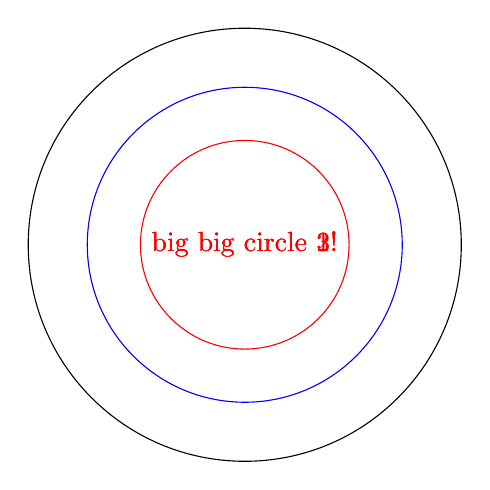
\begin{tikzpicture}
  \node[circle, draw=red, text=red, minimum size=0.5cm] (cbig1) at (0, 0) {big big circle 1!};
  \node[circle, draw=blue, text=red, minimum size=4cm] (cbig2) at (0, 0) {big big circle 2!};
  \node[circle, draw=black, text=red, minimum size=5.5cm] (cbig3) at (0, 0) {big big circle 3!};
\end{tikzpicture}

% -----------------------------------------------------------------------------
\subsection{Anchors and outer sep}
% -----------------------------------------------------------------------------

``anchor=pos'' will anchor the position of the circle to the specified
coordinates. For example, the following nodes anchor the corresponding positions
on the circles to (0, 0).

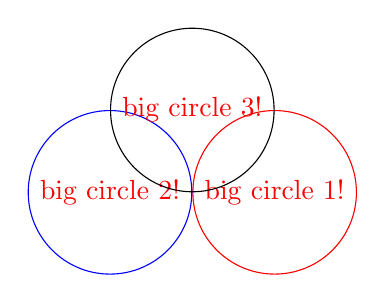
\begin{tikzpicture}
  \node[circle, draw=red, text=red, anchor=west] (cbig1) at (0, 0) {big circle 1!};
  \node[circle, draw=blue, text=red, anchor=east] (cbig2) at (0, 0) {big circle 2!};
  \node[circle, draw=black, text=red, anchor=south] (cbig3) at (0, 0) {big circle 3!};
\end{tikzpicture}

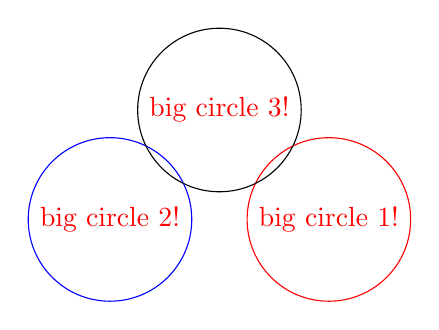
\begin{tikzpicture}
  \node[circle, draw=red, text=red, anchor=west, outer sep=10] (cbig1) at (0, 0) {big circle 1!};
  \node[circle, draw=blue, text=red, anchor=east, outer sep=10] (cbig2) at (0, 0) {big circle 2!};
  \node[circle, draw=black, text=red, anchor=south, outer sep=10] (cbig3) at (0, 0) {big circle 3!};
\end{tikzpicture}

% -----------------------------------------------------------------------------
\subsection{Opacity}
% -----------------------------------------------------------------------------

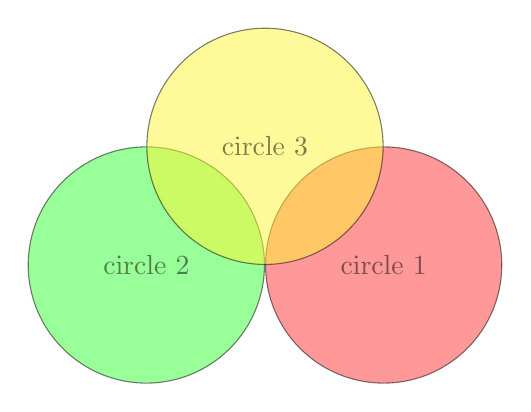
\begin{tikzpicture}
  \node[circle, draw, anchor=west, minimum size=3cm, fill=red!80, opacity=0.5] (cbig1) at (0, 0) {circle 1};
  \node[circle, draw, anchor=east, minimum size=3cm, fill=green!80, opacity=0.5] (cbig2) at (0, 0) {circle 2};
  \node[circle, draw, anchor=south, minimum size=3cm, fill=yellow!80, opacity=0.5] (cbig3) at (0, 0) {circle 3};
\end{tikzpicture}

% =============================================================================
\section{Filling shades of color}
% =============================================================================

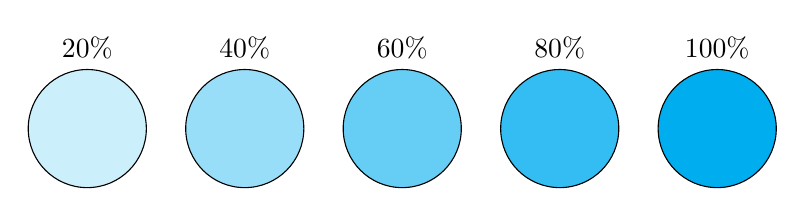
\begin{tikzpicture}

  \foreach \i in {100, 80, 60, 40, 20}{
      \node[draw,
        circle,
        minimum size=1.5cm,
        fill=cyan!\i,
        label={$\i\%$}] (circle1) at (\i/10, 0){};
    }

\end{tikzpicture}

% =============================================================================
\section{Add labels}
% =============================================================================

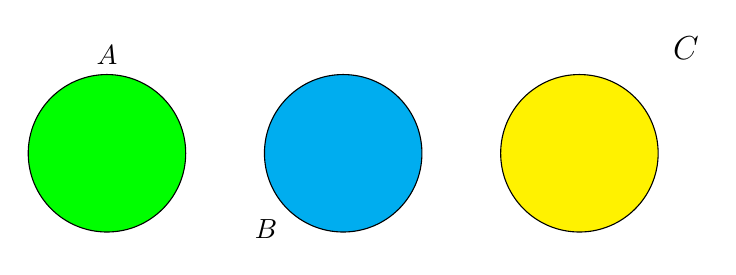
\begin{tikzpicture}

  % Circle with label
  \node[draw,
    circle,
    minimum size=2cm,
    fill=green,
    label=$A$] (circle1) at (0,0){};

  % Circle with label at 225 deg.
  \node[draw,
    circle,
    minimum size =2cm,
    fill=cyan,
    label={225:$B$}] (circle2) at (3,0){};

  % Circle with label at 45 deg and a distance of 0.5cm.
  \node[draw,
    circle,
    minimum size =2cm,
    fill=yellow,
    label={[label distance=0.5cm,font=\large]45:$C$}] (circle2) at (6,0){};

\end{tikzpicture}

% =============================================================================
\section{Draw ellipses}
% =============================================================================

This requires ``shapes.geometric''.

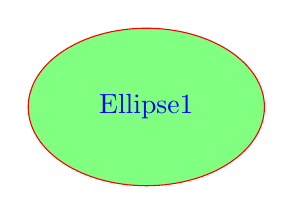
\begin{tikzpicture}

  \node [ellipse,
    draw=red,
    fill=green!50,
    text=blue,
    minimum width = 3cm,
    minimum height = 2cm] (e1) at (0, 0) {Ellipse1};

\end{tikzpicture}

% =============================================================================
\section{Venn diagrams}
% =============================================================================

% -----------------------------------------------------------------------------
\subsection{Simple intersection}
% -----------------------------------------------------------------------------

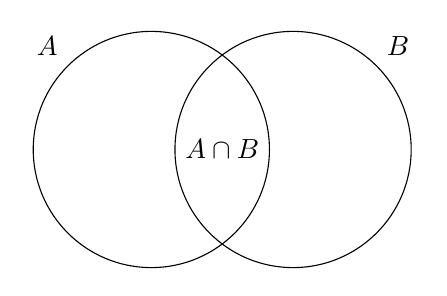
\begin{tikzpicture}

  % Set A
  \node [draw, circle, minimum size=3cm, label={135:$A$}] (A) at (0,0){};

  % Set B
  \node [draw, circle, minimum size=3cm, label={45:$B$}] (B) at (1.8,0){};

  % Set intersection label
  \node at (0.9,0) {$A \cap B$};

\end{tikzpicture}

% -----------------------------------------------------------------------------
\subsection{Simple union with color}
% -----------------------------------------------------------------------------

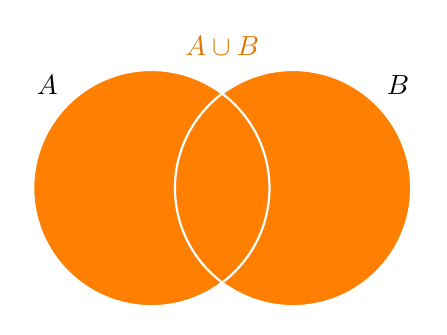
\begin{tikzpicture}

  % Set A
  \node [circle,
    fill=orange,
    minimum size =3cm,
    label={135:$A$}] (A) at (0,0){};

  % Set B
  \node [circle,
    fill=orange,
    minimum size =3cm,
    label={45:$B$}] (B) at (1.8,0){};

  % Circles outline
  \draw[white,thick] (0,0) circle(1.5cm);
  \draw[white,thick] (1.8,0) circle(1.5cm);

  % Union text label
  \node[orange!90!black] at (0.9,1.8) {$A\cup B$};

\end{tikzpicture}

% -----------------------------------------------------------------------------
\subsection{Simple difference}
% -----------------------------------------------------------------------------

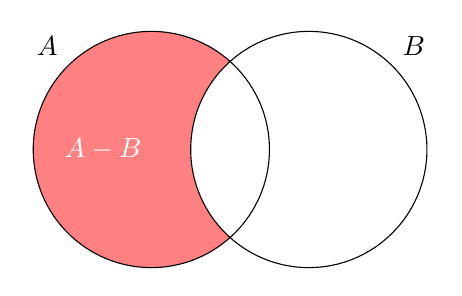
\begin{tikzpicture}

  % Set A
  \node [circle, minimum size=3cm, fill=red!50, label={135:$A$}] (A) at (0,0) {};

  % Set B
  \node[circle, minimum size=3cm, fill=white, label={45:$B$}] (B) at (2,0) {};

  % Circles outline
  \draw (0,0) circle(1.5cm);
  \draw (2,0) circle(1.5cm);

  % Difference text label (note that A's center is used to anchor the label)
  \node[left,white] at (A.center){$A-B$};

\end{tikzpicture}

% -----------------------------------------------------------------------------
\subsection{Intersection with color}
% -----------------------------------------------------------------------------

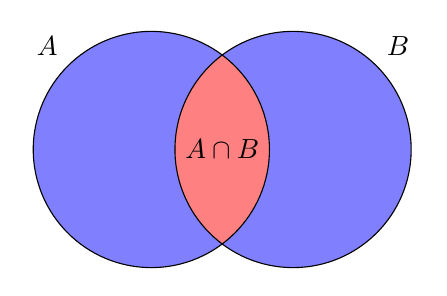
\begin{tikzpicture}

  % Set A
  \node[circle,
    minimum size = 3cm,
    fill=blue!50,label={135:$A$}] (A) at (0,0) {};

  % Set B
  \node[circle,
    minimum size = 3cm,
    fill=blue!50,label={45:$B$}] (B) at (1.8,0) {};

  % Intersection.
  % We used \clip command inside a scope environment to get a local effect of the
  % clipping. All drawings inside the scope environment will be clipped to the
  % closed path created by \clip command. We used \clip twice to consider only
  % the intersection region between the two circles.
  \begin{scope}
    \clip (0,0) circle(1.5cm);
    \clip (1.8,0) circle(1.5cm);
    \fill[red!50](0,0) circle(1.5cm);
  \end{scope}

  % Circles outline
  \draw (0,0) circle(1.5cm);
  \draw (1.8,0) circle(1.5cm);

  % Set intersection label
  \node at (0.9,0) {$A \cap B$};

\end{tikzpicture}

% =============================================================================
\section{Arrows}
% =============================================================================

\begin{tikzpicture}
  \draw [-stealth](0,0) -- (1,0);
  \draw [stealth-](2,0) -- (3,0);
  \draw [stealth-stealth](4,0) -- (5,0);

  \draw [-stealth reversed](0,1) -- (1,1);
  \draw [stealth reversed-](2,1) -- (3,1);
  \draw [stealth reversed-stealth reversed](4,1) -- (5,1);

  \draw [-to](0,2) -- (1,2);
  \draw [to-](2,2) -- (3,2);
  \draw [to-to](4,2)--(5,2);

  \draw [-to reversed](0,3) -- (1,3);
  \draw [to reversed-](2,3) -- (3,3);
  \draw [to reversed-to reversed](4,3)--(5,3);

  \draw [-latex](0,4) -- (1,4);
  \draw [latex-](2,4) -- (3,4);
  \draw [latex-latex](4,4) -- (5,4);
\end{tikzpicture}

\begin{tikzpicture}
  \draw [-latex reversed](0,0) -- (1,0);
  \draw [latex reversed-](2,0) -- (3,0);
  \draw [latex reversed-latex reversed](4,0) -- (5,0);

  \draw [-|](0,1) -- (1,1);
  \draw [|-](2,1) -- (3,1);
  \draw [|-|](4,1) -- (5,1);
\end{tikzpicture}

% =============================================================================
\section{Annotation}
% =============================================================================

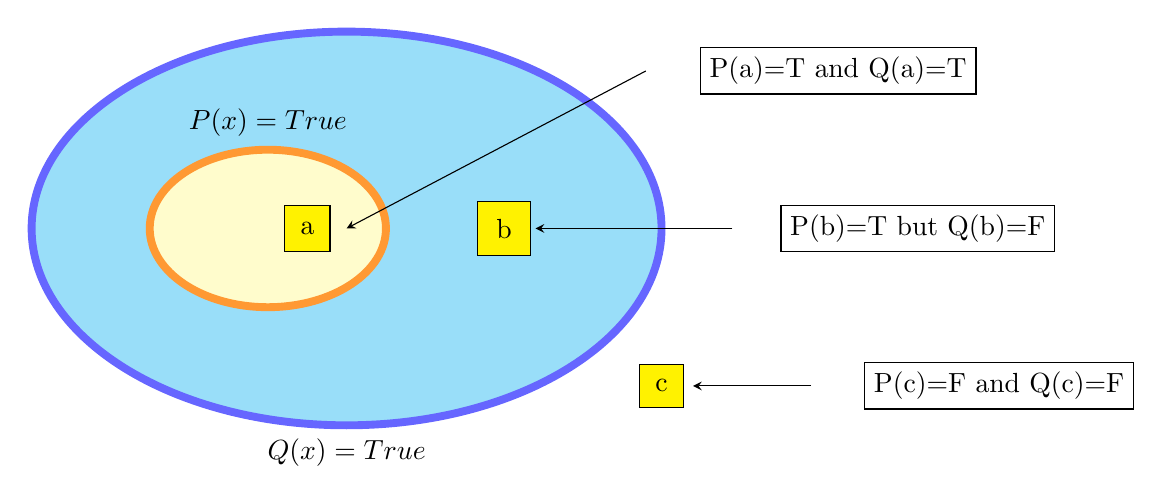
\begin{tikzpicture}
  % Set Q, the enclosing set.
  \node [ellipse,
    draw=blue!60,
    fill=cyan!40,
    line width=1mm,
    minimum width=8cm,
    minimum height=5cm,
    label={-90:$Q(x)=True$}] (Q) at (0,0) {};

  % Set P, the enclosed set.
  \node [ellipse,
    draw=orange!80,
    fill=yellow!20,
    line width=1mm,
    minimum width=3cm,
    minimum height=2cm,
    label={$P(x)=True$}] (P) at (-1,0) {};

  % Element a where P(a) = True and Q(a) = True
  \node [
    regular polygon,
    draw,
    regular polygon sides=4,
    minimum size=0.5cm,
    fill=yellow] (a) at (-0.5,0) {a};
  \node[
    draw=black,
    left, black, fill=white] at (8,2) {P(a)=T and Q(a)=T};
  \draw [-stealth] (3.8,2) -- (0,0);

  % Element b where P(b) = True but Q(b) = False
  \node [
    regular polygon,
    draw,
    regular polygon sides=4,
    minimum size=0.5cm,
    fill=yellow] (b) at (2,0) {b};
  \node[
    draw=black,
    left, black, fill=white] at (9,0) {P(b)=T but Q(b)=F};
  \draw [-stealth] (4.9,0) -- (2.4,0);

  % Element c where P(c) = True and Q(c) = True
  \node [
    regular polygon,
    draw,
    regular polygon sides=4,
    minimum size=0.5cm,
    fill=yellow] (c) at (4,-2) {c};
  \node[
    draw=black,
    left, black, fill=white] at (10,-2) {P(c)=F and Q(c)=F};
  \draw [-stealth] (5.9,-2) -- (4.4,-2);
\end{tikzpicture}

% =============================================================================
\section{Finite Automata and State Diagrams}
% =============================================================================

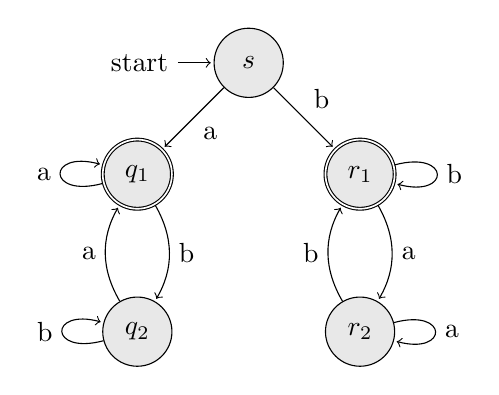
\begin{tikzpicture}[shorten >=1pt,node distance=2cm,auto]
  \tikzstyle{every state}=[fill={rgb:black,1;white,10}]

  \node[state,initial]   (s)                      {$s$};
  \node[state,accepting] (q_1) [below left of=s]  {$q_1$};
  \node[state]           (q_2) [below of=q_1]     {$q_2$};
  \node[state,accepting] (r_1) [below right of=s] {$r_1$};
  \node[state]           (r_2) [below of=r_1]     {$r_2$};

  \path[->]
  (s)   edge              node {a} (q_1)
  edge              node {b} (r_1)
  (q_1) edge [loop left]  node {a} (   )
  edge [bend left]  node {b} (q_2)
  (q_2) edge [loop left]  node {b} (   )
  edge [bend left]  node {a} (q_1)
  (r_1) edge [loop right] node {b} (   )
  edge [bend left]  node {a} (r_2)
  (r_2) edge [loop right] node {a} (   )
  edge [bend left]  node {b} (r_1);
\end{tikzpicture}

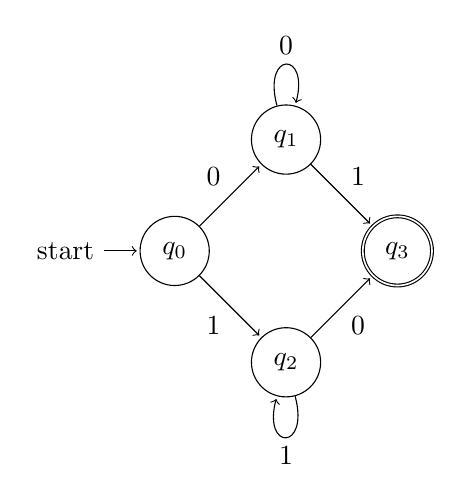
\begin{tikzpicture}[shorten >=1pt,node distance=2cm,on grid,auto]
  \node[state,initial] (q_0)   {$q_0$};
  \node[state] (q_1) [above right=of q_0] {$q_1$};
  \node[state] (q_2) [below right=of q_0] {$q_2$};
  \node[state,accepting](q_3) [below right=of q_1] {$q_3$};
  \path[->]
  (q_0) edge  node {0} (q_1)
  edge  node [swap] {1} (q_2)
  (q_1) edge  node  {1} (q_3)
  edge [loop above] node {0} ()
  (q_2) edge  node [swap] {0} (q_3)
  edge [loop below] node {1} ();
\end{tikzpicture}

How to change the bend angle and edge colors:

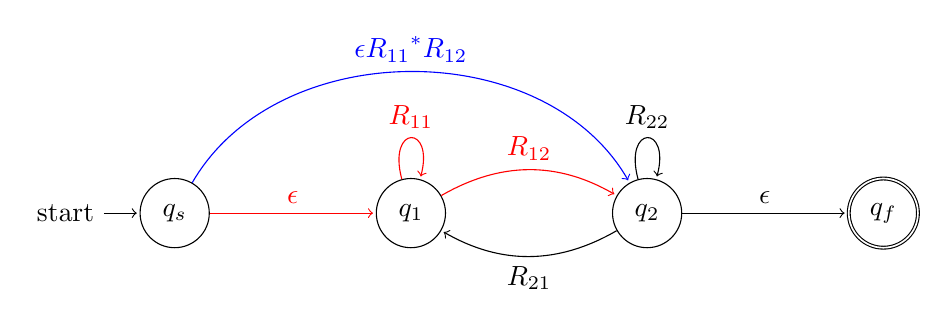
\begin{tikzpicture}[shorten >=1pt,node distance=3cm,auto]
  \node[state,initial]   (q_s)                {$q_s$};
  \node[state]           (q_1) [right of=q_s] {$q_1$};
  \node[state]           (q_2) [right of=q_1] {$q_2$};
  \node[state,accepting] (q_f) [right of=q_2] {$q_f$};

  \path[->]
  (q_s) edge [red]                node {$\epsilon$}                   (q_1)
  (q_s) edge [bend left=60,blue]  node {$\epsilon {R_{11}}^* R_{12}$} (q_2)
  (q_1) edge [loop above,red]     node {$R_{11}$}                     ()
  (q_1) edge [bend left,red]      node {$R_{12}$}                     (q_2)
  (q_2) edge [loop above]         node {$R_{22}$}                     ()
  (q_2) edge [bend left]          node {$R_{21}$}                     (q_1)
  (q_2) edge                      node {$\epsilon$}                   (q_f)
  ;
\end{tikzpicture}

\end{document}
